\subsection{Information}

\indent 

\noindent \textbf{Information}: Collection of data that can be processed, organised, and structured in a meaningful way to convey knowledge, ideas, or instructions.

\bigskip

\noindent Why is \textbf{information important} in IT Professional Practice?

\begin{itemize}
    \item Decision making
    \item Communication with stakeholders
    \item Problem solving and troubleshooting
    \item Project management
    \item Knowledge sharing and continuous learning
    \item Compliance and Ethics
\end{itemize}

\subsubsection{DIKW Hierarchy}

\begin{figure}[h]
    \centering
    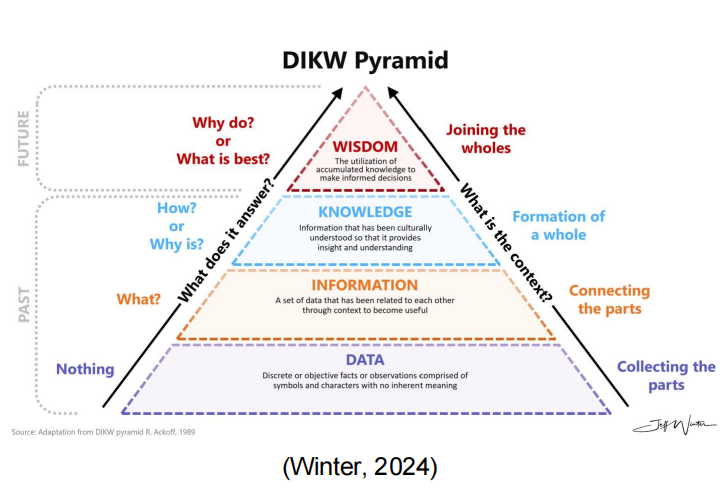
\includegraphics[width=0.7\linewidth]{figures/Week 5/DIKW.png}
\end{figure}

\noindent\textbf{Data}: Raw facts, figures, or symbols without context.

\noindent\textbf{Information}: Processed or organized data that has meaning.

\noindent\textbf{Knowledge}: Applying experience, context, and interpretation to information.

\noindent\textbf{Wisdom}: The ability to make sound judgments and decisions using knowledge.

\subsubsection{What level of information/knowledge is needed?}

\indent 

\noindent\textbf{Data Level}: Needed by technical specialists (e.g., programmers, system admins, analysts) to work with raw logs, records, metrics.

\noindent\textbf{Information Level}: Needed by IT professionals across all roles for decision-making, communication, and reporting. This is the minimum level expected in professional IT practice.

\noindent\textbf{Knowledge Level}: Needed by project managers, consultants, business analysts, senior engineers to interpret and apply information.

\noindent\textbf{Wisdom Level}: Needed by leaders, strategists, architects, and executives for long-term, ethical, and strategic decision-making.

\subsubsection{Why credible information is important?}

\indent 

Credible information is necessary because it ensures \textbf{trustworthy decisions, ethical practice, compliance with laws, and professional accountability}. Without credibility, information loses its value and can even cause harm.

\begin{itemize}
    \item \textbf{Accuracy in Decision}: making Decisions are only as good as the information behind them. Inaccurate or misleading information can lead to costly mistakes, failed projects, or security risks.
    \item \textbf{Trust and professional reputation}: IT professionals work with clients, managers, and users who depend on them. Sharing credible, evidence-based information builds trust and strengthens professional reputation.
    \item \textbf{Risk reduction}: Credible information helps identify risks correctly and avoid poor choices
    \item \textbf{Compliance and Ethics}: Many industries (healthcare, finance, government) require IT professionals to handle verified, accurate information for legal and ethical reasons. Using non-credible information can result in legal breaches, data leaks, or loss of privacy.
    \item \textbf{Efficient Communication}: Teams and stakeholders need a common, reliable source of truth. Credible information ensures everyone is aligned, reducing conflict and confusion.
\end{itemize}

\subsubsection{Sources of Information}

\begin{itemize}
    \item Primary Sources.
    \begin{itemize}
        \item Direct, original, or firsthand evidence.
        \item Example: Research reports, surveys, interviews, company records \& logs, etc
    \end{itemize}
    \item Secondary Sources
    \begin{itemize}
        \item Interpretations, summaries, or analyses of primary data.
        \item Example: Textbooks, documentations, industry reports, news articles, etc.
    \end{itemize}
    \item Tertiary Sources
    \begin{itemize}
        \item Consolidated collections of primary and secondary sources.
        \item Example: Encyclopedias, dictionaries, databases, etc.
    \end{itemize}
\end{itemize}

\subsubsection{Information usefulness vs uselessness}

\indent

\noindent\textbf{Useful Information}: Accurate, Relevant, Timely, Complete, Credible, Understandable, Actionable.

\noindent\textbf{Useless Information}: Inaccurate, Irrelevant, Outdated, Incomplete, Redundant, Unverifiable, Ambiguous.

\subsubsection{What level of information validity is needed?}

\indent

\noindent\textbf{Validity}: The extent to which information is accurate, reliable, and 
represents reality correctly.

\begin{itemize}
    \item \textbf{High} Validity (Critical contexts): Needed when mistakes have serious consequences (legal, financial, ethical, or safety). Example: Medical records, Cybersecurity threat alerts.
    \item \textbf{Moderate} Validity (Operational contexts): Needed for day-to-day IT operations where minor errors can be tolerated but should still be minimized. Example: Project progress reports.
    \item \textbf{Low} Validity (Exploratory/Informal Contexts): Acceptable when using information for brainstorming, trend analysis, or innovation where approximate accuracy is fine. Example: feedback surveys.
\end{itemize}

\subsubsection{How to find information effectively?}

\indent 

\step Define the need: Be clear about what you are looking for.

\step Choose the right sources.

\step Use effective search strategies: Use keywords + Boolean operators (AND, OR, NOT).

\step Evaluate credibility: Use the CRAAP test.

\step Organise and store information: Use reference managers (Zotero, Mendeley, EndNote) and keep structured notes (Evernote, Notion, OneNote)

\step Apply and communicate: Turn raw information into insightful reports, dashboards, or recommendations. Ensure clarity so others can trust and use the information

\subsubsection{CRAAP Test}

\begin{figure}
    \centering
    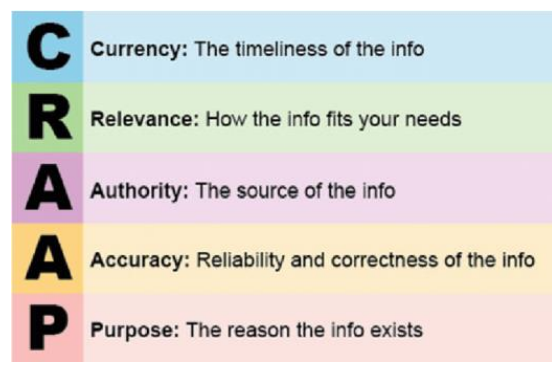
\includegraphics[width=0.7\linewidth]{figures/Week 5/CRAAP.png}
\end{figure}

\begin{itemize}
    \item \textbf{Currency}: Is the information up to date? When was it published or updated?
    \item \textbf{Relevance}: Does the information directly relate to your question or problem? Is it at the right level (too simple / too advanced)?
    \item \textbf{Authority}: Who is the author, publisher, or organization? Are they recognized experts?
    \item \textbf{Accuracy}: Is the information supported by evidence, references, or data? Has it been peer-reviewed or tested?
    \item \textbf{Purpose}: Why was this information created? To inform, teach, sell, persuade, entertain? Is there bias or hidden agenda?
\end{itemize}

\subsubsection{Referencing sources of Information}

\indent

Referencing is how you give credit to the sources of information you’ve used. In IT professional practice and academia, referencing is essential to: 

\begin{itemize}
    \item \textbf{Acknowledge authorship}: avoiding plagiarism.
    \item \textbf{Support credibility}: showing your info is backed by evidence.
    \item \textbf{Allow verification}: so others can find the original source.
\end{itemize}

Common Referencing styles:

\begin{itemize}
    \item \textbf{APA}: Common in IT \& Social Sciences. We use the APA7 format for the assignment.
    \item \textbf{Harvard}: Widely used across disciplines.
    \item \textbf{IEEE}: Standard in engineering, computer science, IT.
\end{itemize}

\subsection{Research}

\indent 

\noindent\textbf{Research}: a systematic process of collecting, analyzing, and interpreting information (data) to answer questions, solve problems, or generate new knowledge.

\bigskip

\noindent Key characteristics:

\begin{itemize}
    \item \textbf{Systematic}: Follows a clear method or process (not random searching).
    \item \textbf{Objective}: Seeks truth or valid results, avoiding personal bias.
    \item \textbf{Evidence based}: Relies on data, experiments, or credible sources.
    \item \textbf{Replicable}: Others should be able to follow the process and reach similar results.
    \item \textbf{Innovative}: Often aimed at discovering new insights or improving existing ones.
\end{itemize}

\subsubsection{Types of Research}

\begin{itemize}
    \item Pure Research: Expands theoretical knowledge (e.g., algorithms, AI models).
    \item Applied Research: Solves practical problems (e.g., developing an HRMS system).
    \item Qualitative Research: Focuses on non-numerical insights (e.g., user experience studies).
    \item Quantitative Research: Uses measurable, numerical data (e.g., system performance benchmarks).
\end{itemize}

\subsubsection{Why research is important in IT?}

\begin{itemize}
    \item \textbf{Innovation and Advancement}: IT evolves rapidly (AI, cloud, cybersecurity, IoT, blockchain). Research drives new technologies, methods, and tools, ensuring professionals stay ahead.
    \item \textbf{Problem Solving}: Research provides systematic approaches to analyze and solve technical or business challenges.
    \item \textbf{Evidence based Decision Making}: Research ensures IT strategies are based on facts, data, and evidence, not assumptions.
    \item \textbf{Improving Professional Practice}: Research identifies best practices, standards, and methodologies (e.g., Agile, ITIL, DevOps).
\end{itemize}

\subsubsection{Primary Research vs Secondary Research}

% Please add the following required packages to your document preamble:
% \usepackage[normalem]{ulem}
% \useunder{\uline}{\ul}{}
\begin{table}[h]
\centering
\begin{tabular}{|c|l|lll|}
\hline
\textbf{Feature}       & \multicolumn{1}{c|}{\textbf{Primary Research}}                                                                                                    & \multicolumn{3}{c|}{\textbf{Secondary Research}}                                                                                                                                  \\ \hline
\textbf{Definition}    & \begin{tabular}[c]{@{}l@{}}Collection of original, first-hand \\ data directly from sources.\end{tabular}                                         & \multicolumn{3}{l|}{\begin{tabular}[c]{@{}l@{}}Use of existing data or information \\ collected by others.\end{tabular}}                                                          \\ \hline
\textbf{Purpose}       & \begin{tabular}[c]{@{}l@{}}To answer specific research \\ questions or problems.\end{tabular}                                                     & \multicolumn{3}{l|}{\begin{tabular}[c]{@{}l@{}}To gather background information,\\ support analysis, or compare findings.\end{tabular}}                                           \\ \hline
\textbf{Sources}       & \begin{tabular}[c]{@{}l@{}}Surveys, interviews, observations,\\ experiments, system logs.\end{tabular}                                            & \multicolumn{3}{l|}{\begin{tabular}[c]{@{}l@{}}Books, journal articles, industry reports,\\ websites, databases.\end{tabular}}                                                    \\ \hline
\textbf{Advantages}    & \begin{tabular}[c]{@{}l@{}}Tailored to your specific research \\ question.\\ Up-to-date and specific.\\ Direct control over quality.\end{tabular} & \multicolumn{3}{l|}{\begin{tabular}[c]{@{}l@{}}Saves time and resources.\\ Provides a broader perspective.\\ Useful for trend analysis and background \\ knowledge.\end{tabular}} \\ \hline
\textbf{Disadvantages} & \begin{tabular}[c]{@{}l@{}}Time-consuming and costly.\\ Requires careful planning and \\ execution.\end{tabular}                                  & \multicolumn{3}{l|}{\begin{tabular}[c]{@{}l@{}}May not be fully relevant or up-to-date.\\ Dependent on the credibility of the \\ original source.\end{tabular}}                   \\ \hline
\textbf{Examples}      & \begin{tabular}[c]{@{}l@{}}Conducting a user survey to test \\ a new HRMS interface.\end{tabular}                                                 & \multicolumn{3}{l|}{\begin{tabular}[c]{@{}l@{}}Reviewing IEEE papers or Gartner reports\\ to learn about cloud security trends.\end{tabular}}                                     \\ \hline
\end{tabular}
\end{table}

\subsubsection{Why statistics matter for research in IT?}

\begin{itemize}
    \item \textbf{Making sense of the Data}: IT research often involves large volumes of data (system logs, user surveys, performance metrics). Statistics provide the tools to analyze, summarize, and interpret this data meaningfully.
    \item \textbf{Turning data into information}: Raw data (primary research) becomes information only when analyzed. Statistics help transform raw counts and numbers into patterns, correlations, and insights.
    \item \textbf{Evidence based decisions}: In IT, decisions about system design, project feasibility, or security risks must be evidence-based. Statistical tests confirm whether findings are valid, reliable, and significant
\end{itemize}

\subsubsection{Important concepts in statistics}

\indent 

\noindent\textbf{Population}: The complete set of items/people/data you are studying.

\noindent\textbf{Sample}: A subset of the population used to make inferences.

\noindent\textbf{Quantitative (Numerical)}: Can be measured and expressed as numbers (e.g., response time, CPU usage).

\noindent\textbf{Qualitative (Categorical)}: Non-numeric, describes qualities (e.g., OS type: Windows, macOS, Linux).

\noindent\textbf{Descriptive}: Summarises data (e.g., mean, median, charts).

\noindent\textbf{Inferential}: Makes predictions or conclusions from data (e.g., hypothesis testing, confidence intervals).

\noindent\textbf{Mean}: Average value.

\noindent\textbf{Median}: Middle value.

\noindent\textbf{Mode}: Most frequent value.

\noindent\textbf{Range}: Difference between max and min.

\noindent\textbf{Variance/Standard Deviation}: How much data points deviate from the mean.

\noindent\textbf{Probability}: The likelihood of an event occurring. Useful in IT for risk assessment, machine learning, and predictive analytics.

\noindent\textbf{Correlation}: : Two variables move together (e.g., internet speed $\uparrow$, user satisfaction $\uparrow$).

\noindent\textbf{Causation}: One variable directly influences another (requires deeper research).

\subsection{Estimation}

\indent 

\noindent\textbf{Estimation}: the process of predicting the effort, time, cost, and resources needed to complete a project or task before the actual work begins.

\bigskip

In IT, estimation is often applied to software development, system implementation, testing, and infrastructure setup.

\subsubsection{Importance of Estimation for IT projects}

\indent

\noindent\textbf{Project Planning \& Scheduling}: 

Accurate estimates allow project managers to plan timelines, set milestones, and allocate resources effectively. Without estimation, projects risk delays and bottlenecks.

\bigskip

\noindent\textbf{Budgeting \& Cost Control}:

Organizations need to forecast project costs for approval and funding. Estimation ensures that financial resources are not over- or under-allocated.

\bigskip

\noindent\textbf{Stakeholder Expectations}:

Helps set realistic deadlines and deliverables for clients, sponsors, and team 
members. Builds trust with stakeholders through transparency.

\bigskip

\noindent\textbf{Resource Management}:

Ensures that human resources (developers, testers, analysts) and technical resources (servers, licenses, tools) are allocated efficiently.

\bigskip

\noindent\textbf{Risk Management}:

Identifies possible overruns early thereby allowing teams to prepare contingency plans.

\bigskip\textbf{Performance Measurement}:

Actual project performance can be compared with estimates to improve future forecasting accuracy.

\subsubsection{5 Steps in Project Estimation}

\indent

\step Determine the \textbf{SIZE} of the project.

This means defining the project scope, functionality, and complexity. In IT, size can be measured using methods like function points, story points, lines of code (LOC), or number of features.

\step Determine the \textbf{EFFORT} required

Effort refers to the total work needed to complete the project. This is typically measured in person-hours, person-days, or person-months. Tools like COCOMO (Constructive Cost Model) or agile estimation techniques can be applied.

\step Decide on the \textbf{RESOURCES} needed

Resources include human (developers, testers, designers), technical (software, hardware, tools), and financial resources. Allocation depends on skill sets required and availability.

\step Calculate the \textbf{DURATION}

Duration is the calendar time required to finish the project given the available resources and effort. Effort and duration are not the same: 100 hours of effort could take 2 weeks with one developer or 1 week with two developers.

\step Calculate the \textbf{COST}

\begin{align*}
    \text{Cost} = (\text{Effort}\times \text{Resource rate}) + \text{Overheads (infrastructure, tools, licenses, etc.)}
\end{align*}

Helps in budgeting and client negotiations.

\subsubsection{5 Approaches to Project Estimation}

\indent 

\noindent\textbf{Function Point Analysis (FPA)}:

Estimates project size by counting the number of “functions” the system must perform (inputs, outputs, user interactions, files, interfaces). Each is given a weight (simple, average, complex).

Good for estimating software development effort where requirements are well-defined.

\bigskip

\noindent\textbf{Algorithmic Cost Models}:

Uses mathematical models based on historical data to estimate effort, cost, and duration. The most famous is COCOMO (Constructive Cost Model).

Usually used in large projects with measurable code size (KLOC = thousands of lines of code).

\bigskip

\noindent\textbf{Expert Judgement}: 

Relies on experienced IT professionals to give estimates based on past-experience.

Used in early-stage projects with uncertain requirements.

\bigskip

\noindent\textbf{Estimation by Analogy}

Compares the project with a similar past project and adjusts based on differences.

Best used when historical projects are available as benchmarks.

\bigskip

\noindent\textbf{Sum of parts}

Breaks the project into tasks or subtasks (like a WBS – Work Breakdown Structure). Each task is estimated separately, then summed up.

Best for detailed project planning when tasks are well-defined.

\subsubsection{Limitations and Biases in Estimation Methods}

\indent 

\noindent\textbf{Function Point Analysis (FPA)}:

\textbf{Limitations}: Can be time-consuming; requires detailed functional specifications early on (which may not always be available).

\textbf{Biases}: Depends on the estimator’s interpretation of system complexity. Different evaluators may assign different function point values.

\bigskip

\noindent\textbf{Algorithmic Cost Models}:

\textbf{Limitations}: Based on assumptions and calibration with historical data; less accurate for novel or emerging technologies.

\textbf{Biases}: “Garbage in, garbage out” - biased or poor-quality input data leads to inaccurate results.

\bigskip

\noindent\textbf{Expert Judgement}: 

\textbf{Limitations}: Relies heavily on personal experience; may not scale well for large, complex projects.

\textbf{Biases}: Subjective optimism (underestimating effort) or pessimism (overestimating effort). Experts may also anchor on past projects that don’t exactly match the current one.

\bigskip

\noindent\textbf{Estimation by Analogy}

\textbf{Limitations}: Requires good historical project data that is truly comparable; differences in scope/technology may be overlooked.

\textbf{Biases}: Over-reliance on similarities, ignoring unique aspects of the new project. May cause “false equivalence bias.”

\bigskip

\noindent\textbf{Sum of parts}

\textbf{Limitations}: Risk of double-counting effort or overlooking hidden dependencies between components

\textbf{Biases}: Anchoring bias if estimators fixate on certain parts while ignoring integration overheads.

\subsubsection{Agile vs Traditional Estimation}

\begin{table}[h]
\centering
\begin{tabular}{|c|l|ll|}
\hline
\textbf{Aspect}      & \multicolumn{1}{c|}{\textbf{Agile Estimation}}                                                                                                                                                                     & \multicolumn{2}{c|}{\textbf{Traditional Estimation}}                                                                                                                                                                                                          \\ \hline
\textbf{Approach}    & \begin{tabular}[c]{@{}l@{}}lterative, adaptive, and based on \\ relative effort.\end{tabular}                                                                                                                      & \multicolumn{2}{l|}{\begin{tabular}[c]{@{}l@{}}Predictive, \\ detailed upfront planning of size,\\ effort, cost, and schedule.\end{tabular}}                                                                                                                  \\ \hline
\textbf{Method}      & \begin{tabular}[c]{@{}l@{}}Uses techniques like \\ Planning Poker, Wideband Delphi,\\ velocity tracking.\end{tabular}                                                                                              & \multicolumn{2}{l|}{\begin{tabular}[c]{@{}l@{}}Uses structured models like COCOMO,\\ Function Point Analysis, \\ Work Breakdown Structures (WBS).\end{tabular}}                                                                                               \\ \hline
\textbf{Focus}       & \begin{tabular}[c]{@{}l@{}}Estimates effort/complexity per feature\\ or user story,\\ not the entire project upfront.\end{tabular}                                                                                 & \multicolumn{2}{l|}{\begin{tabular}[c]{@{}l@{}}Estimates the whole project before\\ execution.\end{tabular}}                                                                                                                                                  \\ \hline
\textbf{Strengths}   & \begin{tabular}[c]{@{}l@{}}Flexible, \\ encourages team collaboration, \\ and provides ongoing re-estimation \\ as the project evolves\end{tabular}                                                                & \multicolumn{2}{l|}{\begin{tabular}[c]{@{}l@{}}Clear budget and timelines commitments\\ at the start. \\ Works well for projects with stable\\ and well-defined requirements.\end{tabular}}                                                                   \\ \hline
\textbf{Limitations} & \begin{tabular}[c]{@{}l@{}}Harder to provide long term \\ cost/duration forecasts. \\ Relies heavily on consistent team\\ velocity and less useful when\\ contracts demand fixed\\ budgets/timelines.\end{tabular} & \multicolumn{2}{l|}{\begin{tabular}[c]{@{}l@{}}Inflexible to changes in requirements \\ and the upfront estimates may become\\ obsolete as the project progresses. \\ There is always a risk of large variances\\ if the assumptions are wrong.\end{tabular}} \\ \hline
\end{tabular}
\end{table}

\subsection{Question}

\subsubsection{End of Lecture Questions}

\begin{itemize}
    \item Why is credible information important for IT professionals?
    \item How does the DIKW hierarchy (Data $\xrightarrow{}$ Information $\xrightarrow{}$ Knowledge $\xrightarrow{}$ Wisdom) help in IT decision-making?
    \item What are the key sources of information, and how can the CRAAP test help evaluate them?
    \item Differentiate between primary and secondary research in IT. Which one would you prefer for a project feasibility study, and why?
    \item Outline the 5 steps of project estimation and explain how they interrelate.
    \item Compare the six approaches to project estimation. Which one is most reliable and why?
\end{itemize}

\subsubsection{Case Study}

\indent 

A mid-sized healthcare company, MediCare Solutions, wants to develop an Electronic Health Record (EHR) system. The system must include:

\begin{itemize}
    \item Patient records storage (structured + unstructured data)
    \item Appointment scheduling
    \item Integration with hospital billing systems
    \item A secure mobile app for patients
\end{itemize}

The CIO assigns a project manager to estimate the project’s size, effort, resources, duration, and cost. The manager must also ensure the information used in the process is valid, credible, and well-researched. They must evaluate estimation methods before deciding.

\bigskip

\noindent\textbf{Question}:

\begin{itemize}
    \item Using the DIKW hierarchy, explain how raw patient data becomes “wisdom” for decision-making in MediCare Solutions.
    \item Identify at least two primary and two secondary research sources the project manager might use in this case.
    \item Apply the five steps of project estimation to the MediCare Solutions EHR system (size, effort, resources, duration, cost).
    \item Which estimation approach (function point analysis, expert judgment, analogy, etc.) would you recommend for this project? Why?
\end{itemize}